\documentclass[10pt,a4paper]{article}
\usepackage[utf8]{inputenc}
\usepackage{amsmath}
\usepackage{amsfonts}
\usepackage{amssymb}
\usepackage{german}
\usepackage{fancyhdr}
\usepackage{graphicx}
\usepackage{geometry}
\usepackage{listings}
\usepackage{hyperref}
\usepackage{color}
\usepackage[usenames,dvipsnames]{xcolor}
\usepackage{DejaVuSans}
\usepackage[T1]{fontenc}
\renewcommand*{\familydefault}{\sfdefault}
\geometry{verbose,a4paper,tmargin=35mm,bmargin=35mm,lmargin=25mm,rmargin=25mm}
\author{Dominik Heeb, Fabian Keller}
\title{Projektplan Semesterarbeit}
\pagestyle{fancy}
\fancyhead{}
\fancyhead[L]{DPC Alrogithmus Vector Clock}
\fancyhead[R]{Domink Heeb, Fabian Keller}
\fancyfoot{}
\fancyfoot[R]{Seite \thepage}

\definecolor{bluekeywords}{rgb}{0,0,1}
\definecolor{greencomments}{rgb}{0,0.5,0}
\definecolor{redstrings}{rgb}{0.64,0.08,0.08}
\definecolor{xmlcomments}{rgb}{0.5,0.5,0.5}
\definecolor{types}{rgb}{0.17,0.57,0.68}
\lstset{language=[Sharp]C,
captionpos=b,
%numbers=left, %Nummerierung
%numberstyle=\tiny, % kleine Zeilennummern
%frame=lines, % Oberhalb und unterhalb des Listings ist eine Linie
showspaces=false,
showtabs=false,
breaklines=true,
showstringspaces=false,
breakatwhitespace=true,
escapeinside={(*@}{@*)},
commentstyle=\color{greencomments},
morekeywords={partial, var, value, get, set},
keywordstyle=\color{bluekeywords},
stringstyle=\color{redstrings},
basicstyle=\ttfamily\normalsize,}

\begin{document}
\begin{titlepage}
	\begin{Huge}
		\begin{center}
				Algorithmus Vector Clock \\Dynamic Parallel Checker\\[2.0cm]
		\end{center}
	\end{Huge}
	
	\begin{center}
		\begin{Large}
				by Dominik Heeb, Fabian Keller\\[1.0cm]
		\end{Large}
		\begin{large}
				Betreuer: Prof. Dr. Luc Bläser
		\end{large}
	\end{center}
\end{titlepage}

\newpage
\tableofcontents 
\newpage

\section{Allgemein}
\subsection{Vector Clock}
\begin{flushleft}
Die Vektor Clock ist ein Vorgehen um einzelnen Messages oder Events einen eindeutigen Zeitstempel zuzuweisen. Somit eine logische Uhr, die es erlaubt in einem Verteilten System (bei uns mehreren Threads) die Ereignisse aufgrund des Zeitstempels einer Kausalordnung zuzuweisen und insbesondere die Nebenläufigkeit von Ereignissen zu ermitteln.
\\[0.5cm]Link:\href{https://de.wikipedia.org/wiki/Vektoruhr}{Wikipedia - Vector clock}
\end{flushleft}
\subsection{Happened-Before Beziehung}
\begin{flushleft}
Ist eine Beziehung zwischen zwei Zeitpunkten. Mit Hilfe der Vektor Clock wird jedem Ereignis ein Zeitstempel zugewiesen und anschliessend herausgefunden in welcher Happened-Before Beziehung die beiden Zeitstempel stehen.\\
Eigenschaften der Happened-Before Beziehung:
\begin{itemize}
\item Auf demselben Prozess: a -> b wenn die Zeit von a < b. (Zeit ist durch lokale Uhr gegeben)
\item Wenn ein Prozess eine Nachricht zu einem anderen Prozess senden, dann a -> b wenn a der Sender und b der Empfänger ist.
\item Für drei Ereignisse a, b, c, wenn a -> b und b -> c, dann a -> c (Transitivität)
\end{itemize}
\end{flushleft}
\newpage
\section{Vector Clock Algorithmus}
\subsection{Beispiel}

\begin{flushleft}
Der Vector Clock Algorithmus wird in diesem Kapitel mit Hilfe von folgendem C\# Code genauer erläutert.\\
\begin{lstlisting}
object a = 1;
object b = 1;
b = 2;
Task.Factory.StartNew(() =>
{
	lock(b) {
		b = 3;
	}
	b = 4;
	lock(a) {
		Console.WriteLine(a);
	}
});
Task.Factory.StartNew(() =>
{
	lock(a) {
		a = 2;
	}
	b = 5;
	lock(b) {
		Console.WriteLine(b);
	}
})
lock(a) {
	a = 3;
}
lock(b) {
	b = 6;
}
Console.WriteLine(a);
\end{lstlisting}
\end{flushleft}

\begin{flushleft}
Diese Beispielfunktion könnte im Ablauf nun wie folgt aussehen:\\[0.5cm]
	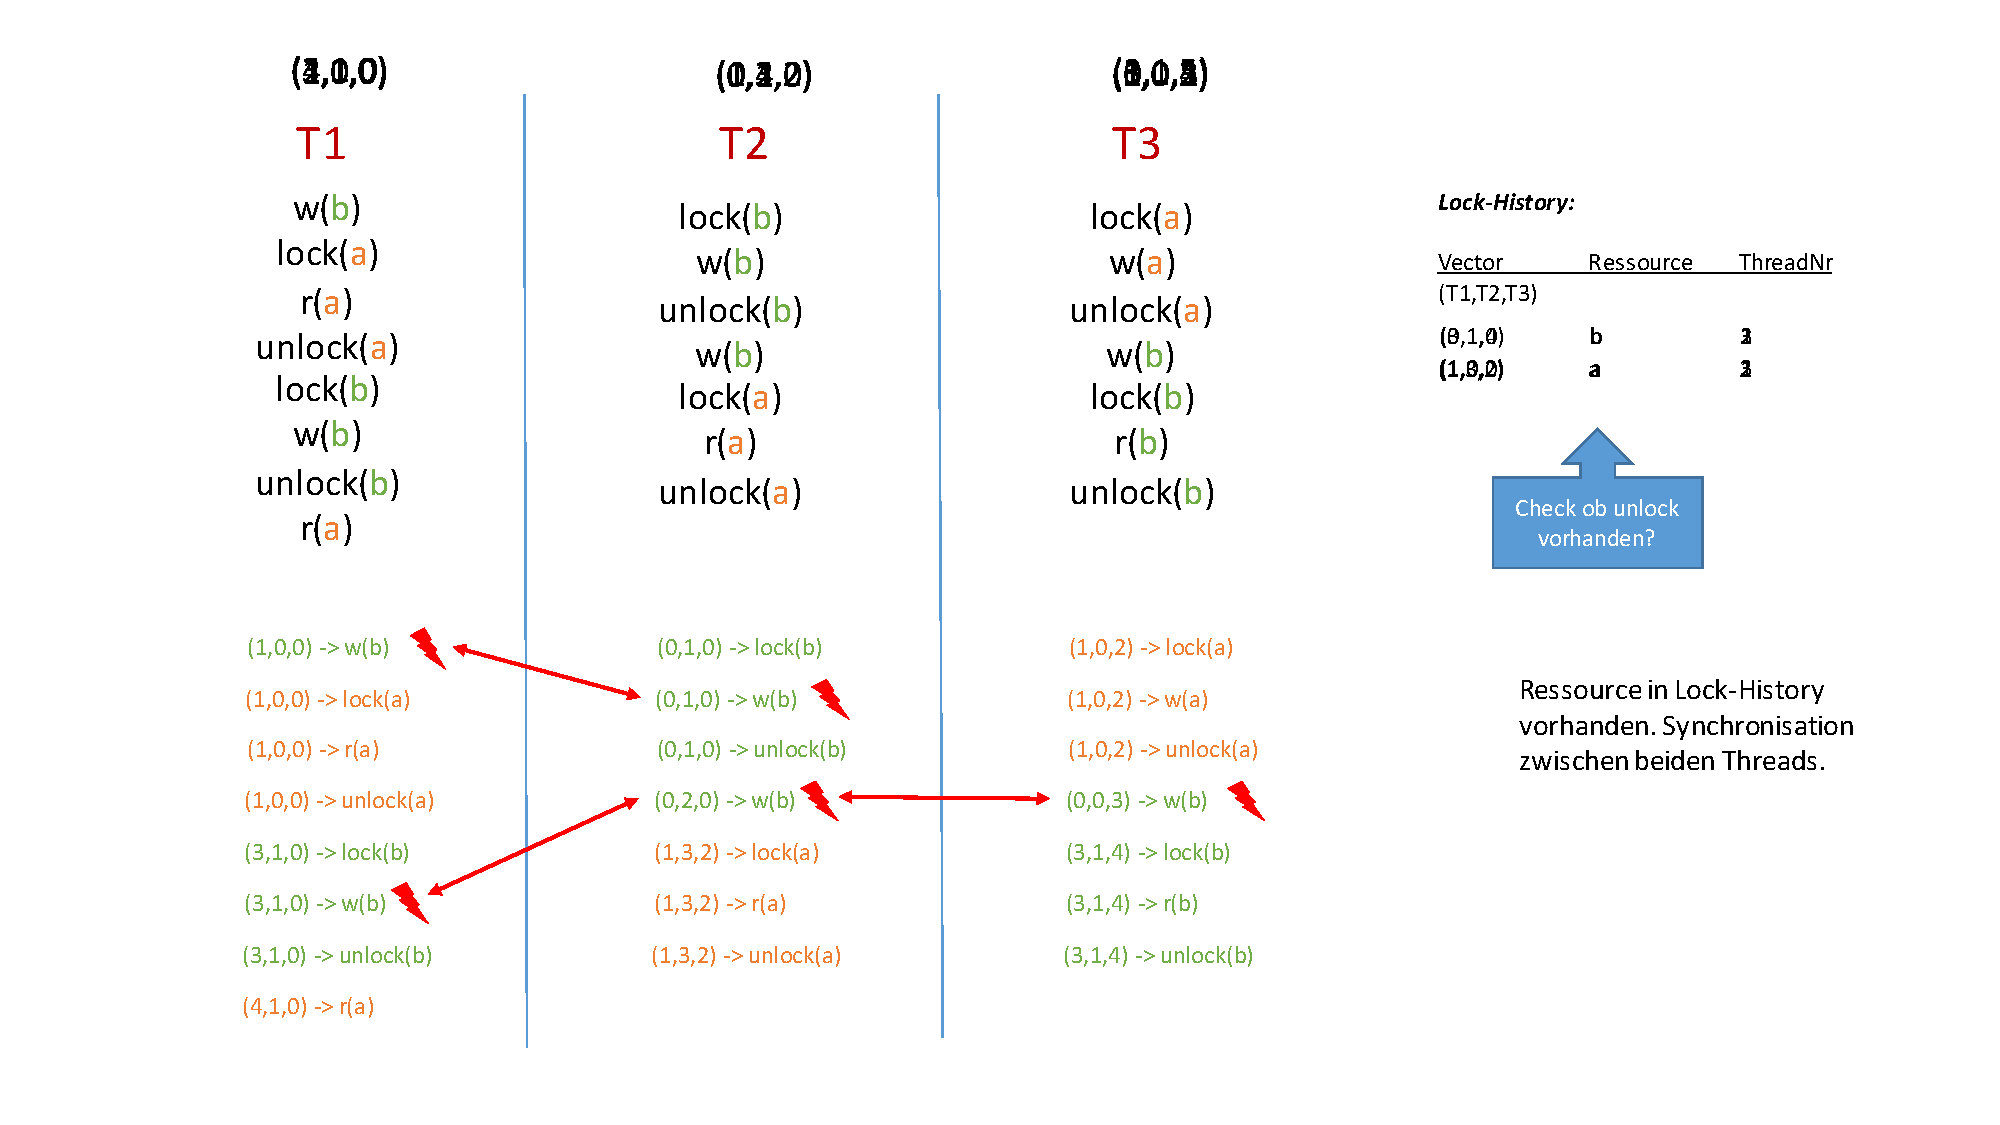
\includegraphics[width=14cm,height=5cm,trim=20mm 90mm 110mm 20mm, clip]{pictures/VectorCheckingAlgorithm.pdf}
\end{flushleft}

\subsection{Vector Clock pro Thread}
\begin{flushleft}
Die Vektor Clock ist eigentlich für verteilte Software Systeme 
\end{flushleft}
\subsection{Funktion}

\begin{flushleft}

\end{flushleft}
\end{document}